\chapter{Holographic Wilson loops}

As discussed in chapter \ref{ch:WilsonLoops}, Wilson loops are important gauge invariant observables 
that can play the role of order parameters of the different phases of the gauge theory.
% Being non-local, there are also natural suggestions for their holographic dual.
Let us describe the basic idea that lead to find the holographic dual of Wilson loops, 
in the context of AdS/CFT correspondence. We then summarize the results obtained for the Pilch-Warner supergravity.


\section{In the $AdS_5 \times S^5$ background}


\subsection{Fundamental representation}
In the fundamental representation, the (Maldacena-)Wilson loop \eqref{maldacenaWL}
describes the phase of a trajectory of an external quark. 
A way to introduce the massive quark is to consider $\mathcal{N}=4$ SYM theory with all the fields in the adjoint representation
of $U(N+1)$ instead.
Then, we break spontaneously the gauge group $U(N+1) \rightarrow U(N) \times U(1)$.
In this way, the off-diagonal states of the scalars that were in the adjoint of $U(N+1)$
become fundamental quarks and anti-quarks in $U(N)$, 
which are massive due to the Higgs mechanism. 
This is a useful picture because, in string theory, 
it is equivalent to separating one D-brane from the original stack of $N+1$ coincident D3-branes.
This produces excited open strings that stretch along the stack and the individual brane,
with the mass proportional to the separation distance. 
Since we consider probe quarks (non-dynamical), the brane must be infinitely far away from the stack.
The stretched strings not only source the gauge fields, but by pulling the $N$ branes, 
they cause deformation on the branes that are described by the scalar fields in \eqref{maldacenaWL}. 
The details of the derivation can be found in the appendix of \cite{Drukker:1999zq}.

Now, let us consider the dual gravitational picture. 
The stack gravitates and the near-horizon geometry is $AdS_5 \times S^5$. 
Then the position of the single D-brane lays on the conformal boundary of $AdS_5$, i.e. $z\rightarrow 0$, 
and sits at a point on $S^5$. 
The probe particle moves on the single D-brane.
The Wilson loop operator is then dual to the partition function of fundamental strings in $AdS_5 \times S^5$ 
whose worldsheets end on the same curve $C$ that defines the Wilson loop at the boundary, \cite{Maldacena:1998im}:
\begin{equation}
 W(C) = \int_{C=\partial \Sigma} DX e^{-S_\text{string}[X]}.
\end{equation}

\begin{figure}[t]
\begin{center}
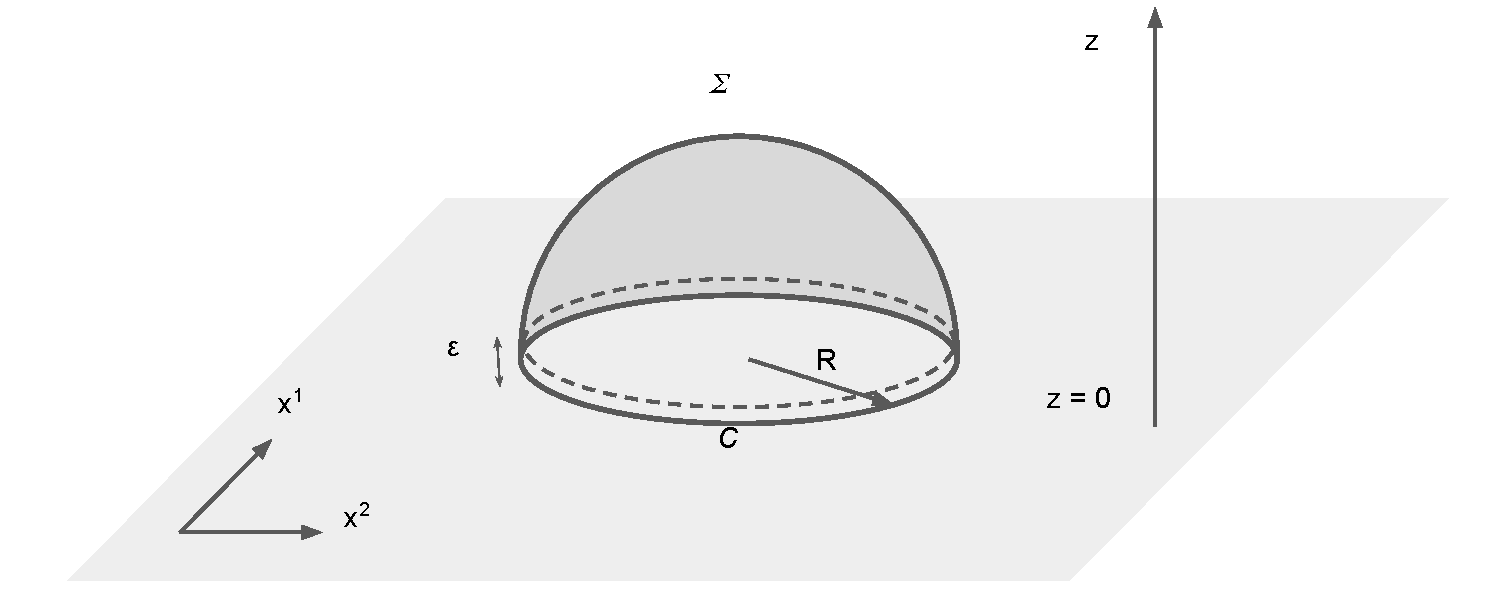
\includegraphics[width=11cm]{Images/WLcircle.pdf}
\end{center}
\caption{\label{fig:WLcircle} Circular Wilson loop as the minimal worldsheet area $\Sigma$ drawn by string ending in the contour $C$ at the boundary of $AdS_5$. }
\end{figure}

In the 't Hooft limit, which corresponds to classical supergravity limit,
minimizing the bosonic string action is sufficient for the leading order, which is essentially the minimal worldsheet area.
% \begin{equation}
%   W(C) \sim e^{-\sqrt{\lambda} A}.
% \end{equation}
Nevertheless, the area is infinite in $AdS$, hence we must regularize it.
For example, the minimal surface that is dual to the circular Wilson loop in the fundamental representation
is parametrized as
\begin{equation}
 z(r)=\sqrt{R^2-r^2}, \quad r\in[0, R], \quad \phi\in[0, 2\pi].
\end{equation}
This result can be obtained either by minimizing the string Nambu-Goto action \cite{Drukker:1999zq},
% \begin{equation}
%  S_\text{NG} = \dfrac{\sqrt{\lambda}}{2\pi} \int d^2 \sigma e^{\Phi/2} \sqrt{\text{det}}
% \end{equation}
or by exploiting the conformal symmetry, i.e. 
mapping the special conformal transformation of the straight line solution \cite{Berenstein:1998ij}.
The induced worldsheet metric, that is the pullback of the background metric $g$ \eqref{metricAdS} in polar coordinates for some $x^i$,
is:
\begin{equation}
 ds^2 = \dfrac{L^2}{z^2}\left((1+z'^2) dr^2 + r^2 d\phi^2 \right).
\end{equation}
Then the on-shell (Nambu-Goto) action gives:
\begin{eqnarray}
 S &=& T_\text{F1} \int \sqrt{\text{det} P[g]}\\
   &=& \dfrac{\sqrt{\lambda}}{2\pi} \int_0^{2\pi} d\phi \int_{0}^{\sqrt{R^2-\epsilon^2}} dr \dfrac{r}{z^2} \sqrt{1+z'^2}\\
   &=& \sqrt{\lambda} \left(\dfrac{R}{\epsilon}-1 \right). \label{minimalAction}
\end{eqnarray}
The correct prescription to regularize the action is to set the boundary cut-off at $z=\epsilon$,
then, we remove the perimeter divergence \cite{Drukker:1999zq}. 
This regularization scheme will be used for other cases of Wilson loop dual computations.
The finite remnant in \eqref{minimalAction} matches with the leading order field theory result \eqref{W1holographic}, i.e.
\begin{equation}
 W_1 = e^{\sqrt{\lambda}}, 
 \quad (N\rightarrow \infty \quad \text{and} \quad \lambda \rightarrow \infty).
\end{equation}

In order to compute the subleading correction 
% $\sqrt{2/\pi}\:\lambda^{-3/4}$ 
in \eqref{W1holographic}, 
the fermionic contribution must be taken into account. 
The full string action to use would be the Green-Schwarz action.
Although it is not fully known in curved background,
its quadratic order is known \cite{Cvetic:1999zs}, which suffices for 1-loop corrections. 
Its quartic order was also derived in \cite{Wulff:2013kga}.
Many efforts have been put into finding the subleading correction  
\cite{Kruczenski:2008zk, Kristjansen:2012nz, Bergamin:2015vxa, Forini:2015bgo, Faraggi:2016ekd, Forini:2017whz}
but no full matching has been achieved.
The ambiguity in the path integral measure hindered this computation.
% A way to evade it was to use the ratio of Wilson loops, and then the matching was proved for the ratio when expanding for small angles \cite{Forini:2017whz}.

\subsection{Higher rank representations}

The lesson from the fundamental Wilson loop suggests that 
the string dual of rank-$k$ representations must be an object that carries $k$ units of the string charge.
Intuitively, if we consider a Wilson loop wrapped $k$ times around the contour (the $k$-fundamental representation), 
we would expect the worldsheet to puff up, due to repulsive charges from multiple coincident fundamental strings.
We see that the individual string action is no longer useful in this case. 
Instead, we can describe the new object in terms of D-branes with fundamental string charges dissolve in it. 
% The charges are the source of a worldvolume electric field in the DBI action (ref).
The worldvolume must also pinch off at the boundary of $AdS_5$, 
ending along the curve defined by the Wilson loop, see figure \ref{fig:WLcircle}.
Supersymmetry will then guide us which D-brane configurations are allowed.


\begin{figure}[t]
\begin{center}
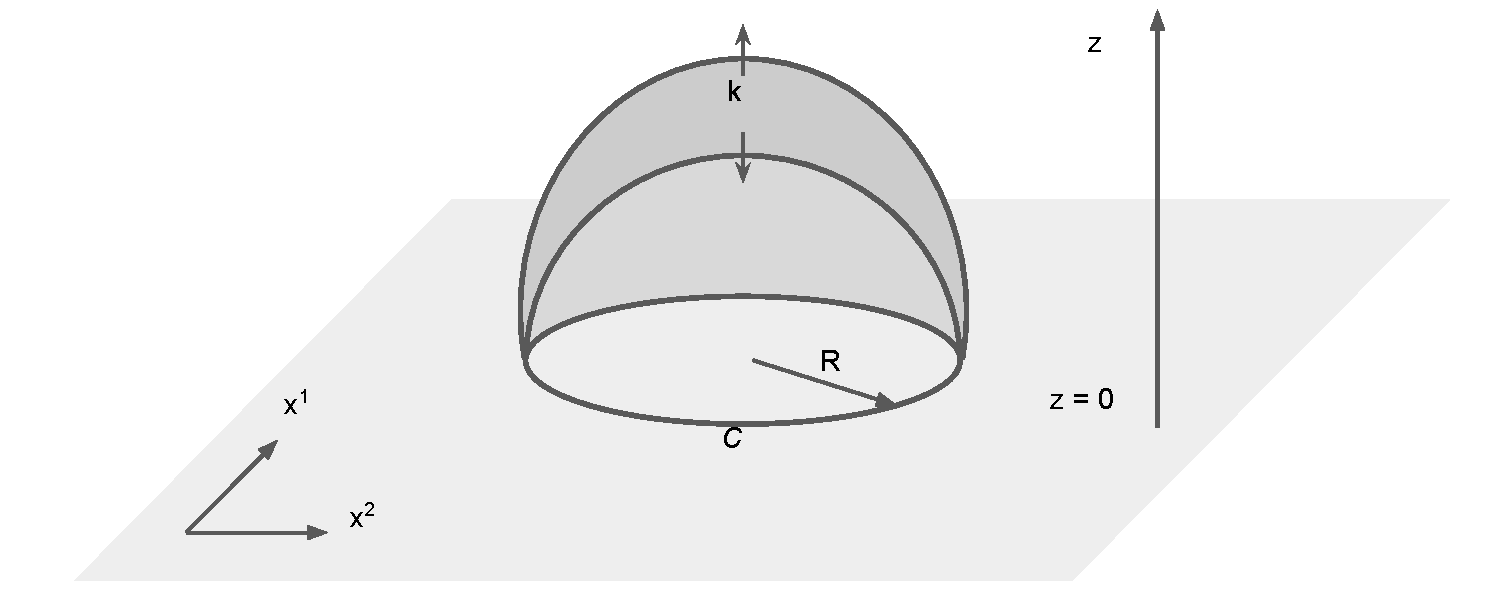
\includegraphics[width=11cm]{Images/DbraneWL.pdf}
\end{center}
\caption{\label{fig:DbraneWL} Circular Wilson loop of rank $k$ as a D-brane with $k$ string charges dissolved in it and the worldvolume ends in the contour $C$ at the boundary of $AdS_5$. }
\end{figure}


More generally, \cite{Gomis:2006sb} related supersymmetric Wilson loops of any representation of the gauge group 
to a stack of bulk D3-branes or a stack of bulk D5-branes, see figure \ref{fig:YoungTable}.
They proved the correspondence by explicitly integrating out the physics on the D-branes, 
which results to a half-BPS Wilson loop insertion in the desired representation in the $\mathcal{N}=4$ SYM path integral.

\begin{figure}[t]
\begin{center}
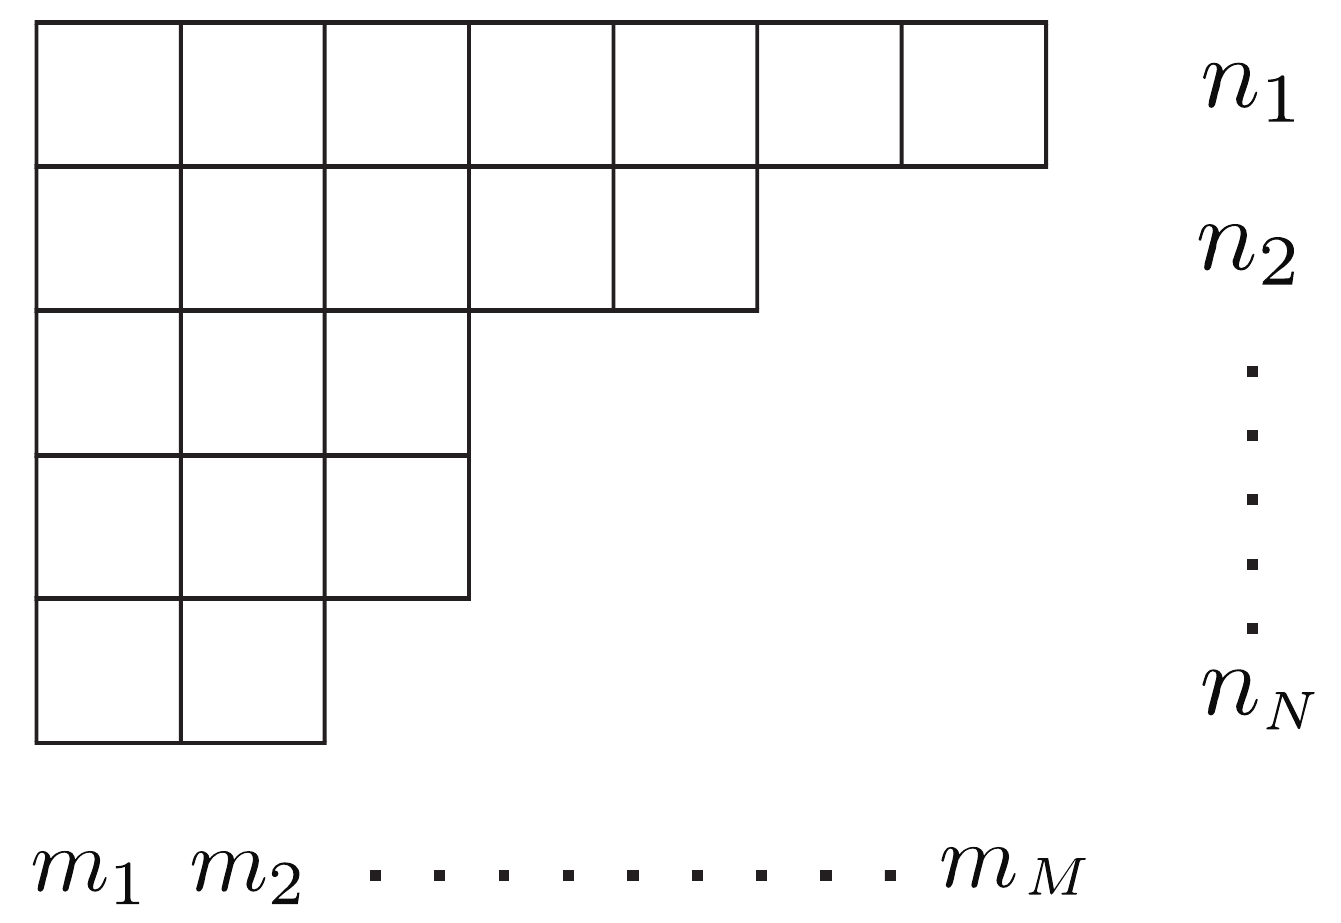
\includegraphics[width=7cm]{Images/YoungTable.png}
\end{center}
\caption{\label{fig:YoungTable} A generic Young table, taken from \cite{Gomis:2006sb}. 
Row $i$ corresponds to a D3-brane with $n_i$ fundamental string charge dissolved in it.
Column $j$ corresponds to a D5-brane with $m_j$ fundamental string charge dissolved in it.
Thus, for symmetric (one row) and antisymmetric (one column) representations,
their rank $k$ corresponds to the string charges a D3-brane and a D5-brane contains.}
\end{figure}

Let us focus on a single D3-brane and a single D5-brane.
Consider first the line element for $AdS_5\times S^5$ is this convenient form:
\begin{equation}
    ds^2 = L^2 \left( du^2 + \cosh^2 u \,d\check{\Omega}^2  + \sinh^2 u \, d\Omega_2^2 
  + d\theta^2 + \sin^2 \theta \, d\Omega_4^2 \right),
\end{equation}
where $u\geq 0$, and $\pi \geq \theta \geq 0 $. 
$d\check{\Omega}_n^2$ and $d\Omega_n^2$ indicate the line element for $AdS_n$ and $S^n$, respectively.
% and we use global coordinates to parametrize $AdS_2$ line element:
% \begin{equation}
%  d\check{\Omega}^2 =d\chi^2+\sinh^2\chi d\varphi^2, \quad \chi\geq 0, \quad 2 \pi \geq \varphi \geq 0.
% \end{equation}
Using the supersymmetry condition\footnote{
May be up to a sign depending on the conventions.}
\begin{equation}\label{susyCondition}
 \Gamma \epsilon =  \epsilon,
\end{equation}
where $\Gamma$ is the kappa symmetry\footnote{
It is a fermionic local gauge symmetry that is present also in particles and strings. 
Its full definition can be found in Paper III.}
projector for the D-brane and $\epsilon$ is the Killing spinor of the background geometry,
we can find the D-brane embeddings that preserve half of the original supersymmetries. 
Note that the supersymmetry condition, which gives first order differential equations,
imply the D-brane equations of motions, which are of second order, up to some integration constants. 
The list below shows the half-BPS D-brane embeddings with their worldvolume geometries
induced from the target space, and the worldvolume gauge fields $F$ \cite{Yamaguchi:2006tq}:
\begin{eqnarray}
 \text{D3-brane:} &\quad& AdS_2 \times S^2, \quad u=\text{constant}, \quad \theta = 0 \\
		  &\quad& \dfrac{1}{T_{F1}}F = L^2\sqrt{1+\kappa^2} e^0 e^1, \quad \kappa \equiv \sinh u \\
 \text{D5-brane:} &\quad& AdS_2 \times S^4, \quad u=0, \quad \theta = \text{constant} \\
 		  &\quad& \dfrac{1}{T_{F1}}F = L^2 \cos \theta e^0 e^1 
\end{eqnarray}
where $e^0$ and $e^1$ are the vielbeins\footnote{
Vielbeins are defined by $ds^2=\eta_{mn} e^m e^n$, which is often referred as the \emph{local frame}.
In terms of components: $e^m=e^m_M dx^M$, thus, we can relate them to the metric as $g_{MN} = \eta_{mn} e^m_M e^n_M$.} 
of $d\check{\Omega}^2$. 
We see that the D3-brane sits on a fixed point on the $S^5$, 
while the D5-brane sits on $S^4$ that is $\theta$ angle away from the pole of $S^5$, see figure \ref{fig:S5}.


\begin{figure}[t]
\begin{center}
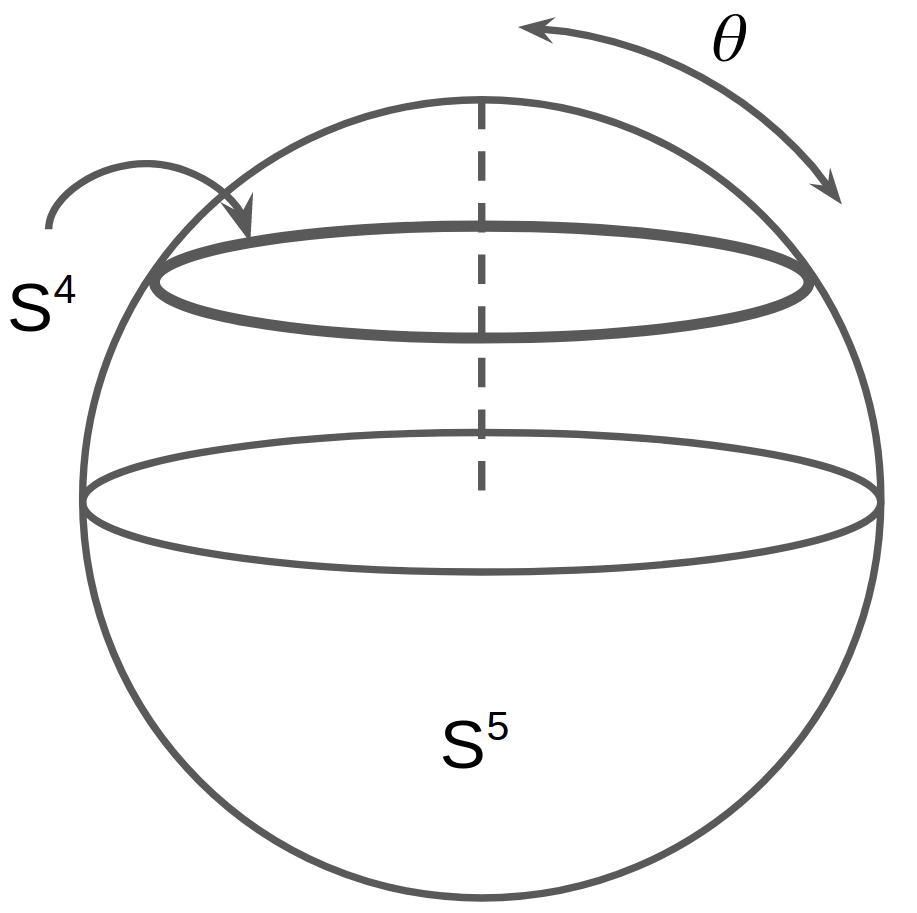
\includegraphics[width=4cm]{Images/S5.png}
\end{center}
\caption{\label{fig:S5} $S^4$ that is $\theta$ angle away from the pole of $S^5$. 
The angle depends on the amount of string charges $k$ that D5-brane contains.}
\end{figure}


The dual counterparts of the symmetric/antisymmetric representation in the leading order 't Hooft limit
are the on-shell action DBI \eqref{DBI} + WZ \eqref{WZ} of the D3-brane/D5-brane configuration aforementioned:
\begin{equation}\label{WLDbrane}
 \log W^{+}_k = - S_{D3}, \quad \log W^{-}_k = - S_{D5}.
\end{equation}
Moreover, we must ensure the string charge $k$ constraint, which can be added as a Lagrange multiplier term to the D-brane action:
\begin{equation} \label{stringChargeConstraint}
S_k = - k  \int_\Sigma F 
\quad \Rightarrow \quad  
k = \dfrac{1}{T_{F1}} \dfrac{\delta S_\text{DBI}}{\delta F} .
\end{equation}
The couplings in terms of $\lambda$ and $N$ are:
\begin{equation}
 T_\text{F1} = \dfrac{\sqrt{\lambda}}{2\pi L^2},
 \quad
%  T_\text{D1} = \dfrac{2N}{\sqrt{\lambda}},
%  \quad 
 T_\text{D3} = \dfrac{N}{2\pi^2 L^4},
 \quad 
 T_\text{D5} = \dfrac{N\sqrt{\lambda}}{8\pi^4 L^6},
\end{equation}
which are derived from \eqref{couplingsTension} using \eqref{couplings}.

Finally, the regularized actions are \cite{Drukker:2005kx, Yamaguchi:2006tq, Zarembo:2016bbk}: 
\begin{eqnarray}
 S_\text{D3} &=& - 2 N  (\kappa\sqrt{1+\kappa^2}+\mathop{\mathrm{arcsinh}}\kappa)\\
 S_\text{D5} &=& - N \frac{2\sqrt{\lambda }}{3\pi}\,\sin^3\theta,
\end{eqnarray}
with the $\theta$ satisfying the string charge constraint \eqref{stringChargeConstraint} that gives \eqref{eqThetaAntisym}, i.e. 
\begin{equation}
 \theta -\frac{1}{2}\,\sin 2\theta =\pi \frac{k}{N}.
\end{equation}
Thus the latitude angle $\theta$ depends on the amount of string charges $k$ dissolved in the D5-brane.
In conclusion, there is an exact agreement with \eqref{solW+} and \eqref{solW-}, according to \eqref{WLDbrane}.



\section{In Pilch-Warner background}

In $\mathcal{N}=2^*$ SYM on $S^4$, we took the decompactification limit for circular Wilson loops in order to have results on $\mathbb{R}^4$.
This means that in the Pilch-Warner background, the contour is a straight line of length $l\rightarrow \infty$. 

\subsection{Fundamental representation}
The minimal surface of a straight Wilson line is a wall,
with the worldsheet coordinates $(\tau, \sigma)$ induced from the Pilch-Warner geometry in the following way:
\begin{equation}
 \tau = x^1, \quad \sigma = c.
\end{equation}
The regularized on-shell action was computed in \cite{Buchel:2013id}, 
which agrees with the leading order result in \eqref{WLFundN2}, that is:
\begin{equation}\label{W1leading}
 \log W_1 = \sqrt{\lambda} M \frac{l}{2\pi }, \quad (l\rightarrow \infty).
\end{equation}


The goal of Paper V was to compute the loop corrections to the minimal surface 
by using string perturbation around the above classical solution.
There are two contributions, which turned out to be of equal weight in our case. 
The first one comes from the dilaton coupling to the worldsheet curvature called the Fradkin-Tseytlin term \cite{Fradkin:1983xs}:
\begin{equation}
 S_{FT}=\dfrac{1}{4\pi} \int d^2\sigma \sqrt{h}  R^{(2)} \Phi,
\end{equation}
which is actually a bit controversial, 
with some authors arguing it is not needed \cite{GRISARU1988625, GRISARU1985116, Cvetic:1999zs}.
Besides, it is zero for the familiar $AdS_5 \times S^5$ background due to a vanishing dilaton. 
% explicitly break the conformal invariance of the classical world-sheet action
The other one comes from 1-loop stringy corrections, 
which are computed by expanding the Green-Schwarz action up to quadratic fluctuations \cite{Cvetic:1999zs}.
These contribute as functional determinants, from generalizing the Gaussian integration formula \eqref{GaussianIntegral} for the bosons,
and the Grassmann integration for the fermions \eqref{GrassmannIntegral}.
Thus the semiclassical partition function is schematically of the form
\begin{equation}
 W = e^{-S_\text{cl}-S_\text{FT}} \dfrac{\text{det} F}{\sqrt{\text{det} B}},
\end{equation}
where $S_\text{cl}$ is the classical on-shell action in \eqref{W1leading}, 
$B$ and $F$ here just represent the bosonic and fermionic operators.
% of Schroedinger type (second order differential operator), 
% of Dirac type ($2\times2$ first order differential operator). 

Supersymmetry simplifies our problem by cancelling exactly 
the sector of bosonic and fermionic operators that are asymptotically massless (far away from the boundary $\sigma=1$).
The remaining sector is asymptotically massive, and the operators (after several manipulations) look enticingly similar:
\begin{equation}\label{basicDirac}
 H_B=\begin{pmatrix}
  1+\frac{A}{\sigma }  & \mathcal{L} \\ 
  \mathcal{L}^\dagger  & -1 \\ 
 \end{pmatrix},\qquad 
  H_F=\begin{pmatrix}
  -1                   & \mathcal{L} \\ 
  \mathcal{L}^\dagger  & 1+\frac{A}{\sigma }  \\ 
 \end{pmatrix},
\end{equation}
with
\begin{eqnarray}\label{EuclideanLs}
 \mathcal{L}&=&A\sqrt{\sigma ^2-1}\,\partial _\sigma +\frac{A\left(2\sigma ^2+1\right)}{2\sigma \sqrt{\sigma ^2-1}} ,
\nonumber \\
 \mathcal{L}^\dagger &=&-A\sqrt{\sigma ^2-1}\,\partial _\sigma 
-\frac{A\left(4\sigma ^2-1\right)}{2\sigma \sqrt{\sigma ^2-1}}
+\frac{2}{\sqrt{\sigma ^2-1}}\,.
\end{eqnarray}
The final semiclassical partition function to compute is then:
\begin{equation}\label{semiclassicalW}
  W = e^{-S_\text{cl}-S_\text{FT}}\dfrac{\text{det}^2 (\partial_\tau-H_F)}{\text{det}^2 (\partial_\tau-H_B)},
\end{equation}


Instead of using the heat kernel technique or the Gelfand-Yaglom method, 
both commonly used in the computation of functional determinants,
we used the phase-shift method from quantum mechanical scattering problems, see e.g. \cite{PhysRevD.10.4130}.
The method requires the operators to be asymptotically free, hence it works for (semi-)infinite intervals.
Our operators \eqref{basicDirac} share the same asymptotics in large $\sigma$, and they are defined in a semi-infinite interval $\sigma>1$,
so the method applies. Note that for $\tau$ variable, we do a usual Fourier transformation. 
The exponential of the ratio of the determinants of the operators in \eqref{semiclassicalW}
can be written in terms of the phase-shift $\delta(p)$ between the wave function and the asymptotic plane wave, 
see figure \ref{fig:potentialWavesPlot},
which is
\begin{equation}\label{deltaphases}    
 -2 \, \int_{0}^{\infty }\frac{dp}{2\pi }\,\,
 \frac{4 p }{9\sqrt{\frac{4}{9}\,p^2+1}}\,\left(
 \delta_F ^+(p)
 +
\delta_F ^-(p)
-\delta_B ^+(p)
 -
\delta_B^-(p)
\right) = -\dfrac{1}{4},
\end{equation}
where $\pm$ distinguish the two eigenvectors (particles and holes) of the Dirac Hamiltonians \eqref{basicDirac}.
The last equality is backed by our numerics.
Thus, together with the Fradkin-Tseytlin contribution, the total correction is $-1/2$. 
In conclusion, we do have a perfect matching with the field theory result \eqref{WLFundN2}.
% up to the subleading order in strong coupling expansion.
Moreover, the existence of Fradkin-Tseytlin term is necessary for this agreement.




\begin{figure}[t]
\begin{center}
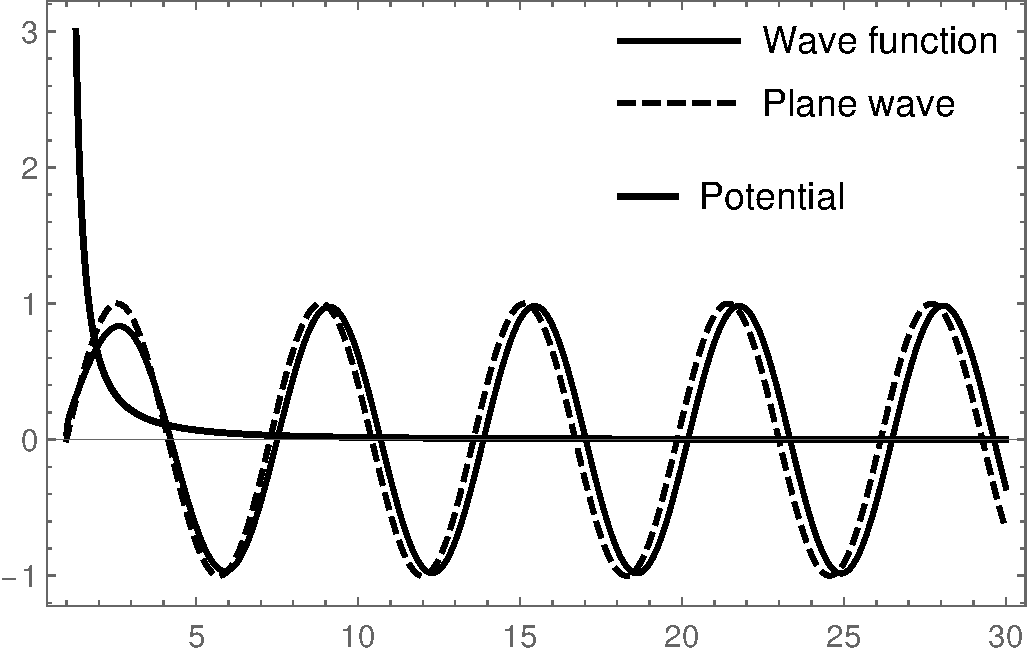
\includegraphics[width=0.7\textwidth]{Images/potentialWavesPlotBlack.pdf}
\end{center}
\caption{\label{fig:potentialWavesPlot} Phase-shift $\delta(p)$ of the wave function 
in the presence of a typical potential wall that many of our operators show, versus the free wave, 
for certain momentum $p$. 
}
\end{figure}


\subsection{Symmetric representation}
As for higher rank Wilson loops, Paper III found the D3-brane embedding dual to 
the straight Wilson line of length $l$ in symmetric representation, with the help of the supersymmetric condition \eqref{susyCondition}. 
The worldvolume metric is induced from the deformed $AdS$ part of \eqref{metricPW} in string frame\footnote{
We changed to mostly minus signature in order to follow Paper III.
The string metric $g$ and the Einstein metric $G$ are related by $g=e^{-\frac{4 \Phi }{D-2}} G$,
where $\Phi$ is the dilaton. 
}:
\begin{equation}
 ds^2 = \dfrac{A M^2 L^2}{c^2-1}\left(dx^2  - \rho(c)^2 d\Omega_2^2 \right)
	-L^2\left(\dfrac{1}{A \left(c^2-1\right)^2} + \dfrac{A M^2 \rho'(c)^2}{c^2-1} \right) dc^2,
\end{equation}
where 
\begin{equation}
 \rho(c)= \kappa \, \sqrt{c^2-1},
\end{equation}
since the deformed sphere shrinks to $\theta=\pi/2$ and $\phi=0$.
The worldvolume gauge field is given by
\begin{equation}
 \frac{1} {T_\text{F1}} F (c)  = -\dfrac{M L^2}{(c^2-1)^{3/2}} dx\wedge dc.
\end{equation}
As expected, it also reduces to the analogous case in $AdS_5 \times S^5$ close to the boundary. 

The regularized on-shell action reduces to
\begin{equation}
 S_{D3} = - \sqrt{\lambda} k M \dfrac{l}{2\pi}.
%  , \quad (l \rightarrow \infty).
\end{equation}
This agrees with the matrix model result \eqref{WsymPW} according to \eqref{WLDbrane}, only in the low rank limit
\begin{equation}
 \kappa \ll M l.
\end{equation}
Furthermore, for $k=1$, we recover the fundamental case \eqref{W1leading}.
We can conclude that this D3-brane configuration cannot probe the entire matrix model region, 
and a full dual object is still to be understood.

For the antisymmetric case, it is technically challenging to find the D5-brane solution. 
So far, we have not succeeded.
We do expect it though to match the leading order field theory result, 
because the matrix model result \eqref{WantisymPW} is proportional to $Ml$, the same as in the D-brane action.
It would be definitely interesting to compute the subleading order to determine the phase-transitions observed. 


